\documentclass{article}
\usepackage{hyperref}
\usepackage{listings}
\usepackage{graphicx}
\usepackage{fancyhdr}
\usepackage{color}
\usepackage{float}

\pagestyle{fancy}



\begin{document}


\begin{titlepage}
	\begin{center}
	\line(1,0){300}\\
	[0.25in]
	\huge\bfseries\ Programming Project 3 \\Gnutella-style peer-to-peer (P2P) file sharing system \\
	
	
	\line(1,0){250}\\
	\bfseries {Geoffrey Rathinpandi}\\
	\end{center}
	
	

	\begin{flushright}
	\textsc{R11488765}\\
	
	
	\end{flushright}
	\tableofcontents
\end{titlepage}
\section{GithubLink}
The github link :  \url{https://github.com/Ge0f3/Gnutella-peer-peer } \\ \\

\section{Overview}

This project aims to provide a Gnutella -style peer-to-peer file sharing system.In which each peer will act as both client as well as a server.As a server, it accepts queries from other peers, checks for matches against its local data set and responds with results.As a client, it provides interfaces through which users can issue queries and view search results.In addition to this project since there is no central indexing server search is done in a distributed manner. Each peer maintains a list of neighboring peers whenever a query request comes in the peer will broadcast the query to all its neighbors in addition to searching its local storage and responds.


\section{Architecture}

There are two type of design implementation used in Gnutella  \\
\begin{itemize}
\item Star Topology
\item Mesh Topology
\end{itemize}

\subsection{Star Topology}
In star topology peer one is placed in the middle while the others are connected statically to peer one
\begin{figure} [H]
\centering
        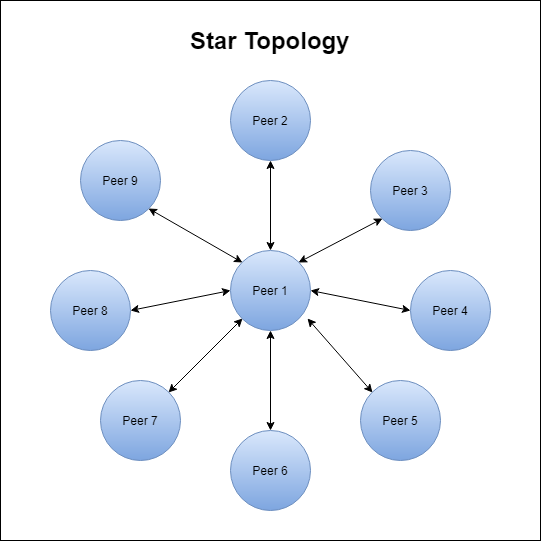
\includegraphics[totalheight=8cm]{starArch.png}
    \caption{Star Topology}
    \label{fig:verticalcell}
\end{figure}

\textbf{Config File}

Below is the config file of Star Topology

\begin{figure} [H]
\centering
        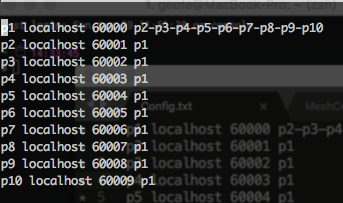
\includegraphics[totalheight=8cm]{Star.png}
    \caption{Mesh Topology}
    \label{fig:verticalcell}
\end{figure}

\subsection{Mesh Topology}
In mesh topology peers are placed in a 2D-mesh and  each peer is interconnected with one another.
\begin{figure} [H]
\centering
        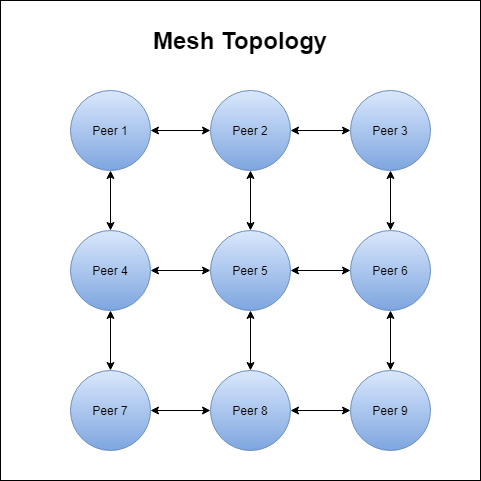
\includegraphics[totalheight=8cm]{MeshArch.png}
    \caption{Mesh Topology}
    \label{fig:verticalcell}
\end{figure}

\textbf{Config File}

Below is the config file of Mesh Topology
\begin{figure} [H]
\centering
        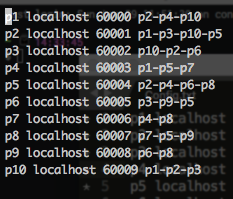
\includegraphics[totalheight=8cm]{Mesh.png}
    \caption{Mesh Topology}
    \label{fig:verticalcell}
\end{figure}


\section{Implementation}
When a user query a search request for a file, he will send a broadcast message to his neighbours who are going to do the same if they do not own the requested file.
If a file found, the file owner will send back a hit query the requester through the addresses that have been stored in the header message of all passby nodes.
If a node received the same message one more time, it will drop it immediately. This action is done by doing the following steps:
\begin{itemize}
\item 1. When a new message created, attache the PK (peer ID+time stamp) along with message, and store it in the PK field.
\item 2. For any broadcasted message, record the PK in a list.
\item 3. For every received message, compare the PK with the stored PKs. If found, drop the message.
\end{itemize}

Else, broadcast the message.


\section{Future Enhancement}
\begin{itemize}
\item Enhancing the performance by apply load balancing approach on the server side.
\item Dynamic ports allocation needed in the system to avoid overlapping reserved
ports.
\item A simple GUI will make it user friendly.

\end{itemize}





\end{document}